\documentclass[UTF8,a4paper,landscape,16pt]{paper}
\usepackage{ctex}
\usepackage{amsmath}
\usepackage{pdfpages}
\usepackage{graphicx}
\usepackage{wrapfig}
\usepackage{listings}
\usepackage{xcolor}
\usepackage{multicol}
\usepackage{float}
\usepackage{flushend}
\usepackage{cuted}
\usepackage{fancyhdr}
\usepackage[utf8]{inputenc}
\usepackage[landscape]{geometry}
\usepackage[figuresright]{rotating}
\linespread{0.5}
\geometry{left =0cm,right = 0cm,top = 0cm, bottom = 0cm}
\pagestyle{fancy}
\begin{document}\footnotesize
\begin{multicols}{4}
\section{命题逻辑}
\subsection{命题,命题公式}
\noindent 命题:能判断真假(不是既真又假)的陈述句为命题。如:“雪是黑色的”,一般由小写英文字母p,q,r,s等表示。

\noindent 单个常量或变量的命题称作合式公式;联结词联接的合式公式的组合也是合式公式;合式公式有限次的组合所构成的字符串成为命题公式.习惯上用大写英文字母A,B,C,D等表示

\noindent \\lnot{}否定(非), $\land$合取(与),$\lor$析取(或),$\rightarrow$ 蕴含(IF...THEN) ,$\leftrightarrow$等价(当且仅当)

\noindent 命题公式的联结词组合仍然是命题公式,$A\rightarrow B$只有A取T,B取F时结果才为F

\noindent 给命题中的各变量赋值成为对该命题的一个解释,若公式中命题变量由p,q,r给出,则顺序由英文字母顺序给出,真值表:设公式 A含$n(n \ge 1)$ 个命题变量,将 A在$2^{n}$个取值下的取值情况列成表,称为 A的真值表。公式的分类:永真式(全1)、永假式(全0)、可满足式(可1)、非重言式的可满足式(可1可0)

\noindent $A \rightarrow B \Leftrightarrow \lnot A \lor B,\text{  置换规则可以充分使用}\\  A \leftrightarrow B \Leftrightarrow (A \rightarrow B)\land (B \rightarrow A),\\ A\rightarrow B \Leftrightarrow \lnot B \rightarrow \lnot A,\\  A \leftrightarrow B \Leftrightarrow \lnot A \leftrightarrow \lnot B,\\  (A\rightarrow B) \land (A\rightarrow \lnot B) \Leftrightarrow \lnot A,\\ A \Rightarrow (A\lor B),\ (A\land B) \Rightarrow A,\\ ((A\rightarrow B) \land A) \Rightarrow B,\ ((A\rightarrow B)\land \lnot B) \Rightarrow\lnot A,\\ ((A\lor B)\land \lnot A) \Rightarrow B,\\ ((A\rightarrow B) \land (B \rightarrow C)) \Rightarrow (A\rightarrow C),\\ ((A\leftrightarrow B) \land (B \leftrightarrow C)) \Rightarrow (A\leftrightarrow C),\\ (A\rightarrow B) \land (C \rightarrow D) \land (A\lor C) \Rightarrow (B \lor D)$

优先顺序 $\lnot$高于$\land\lor$高于$\leftrightarrow\rightarrow$,括号优先,同级从左向右

\noindent 任意命题公式都存在着与之等值的析取范式和合取范式。

\noindent 求合取范式的基本原则:利用$\lor$对$\land$的分配。(将$\land$移动到外面来),基本步骤:
\begin{itemize}
\item 削去对于$\lnot,\lor,\land$来说冗余的联结词;
\item 内移或削去否定号;
\item 利用分配率。
\end{itemize}

\noindent 归结原理:$p \lor q\land\lnot q \lor r\Rightarrow p \lor r$.

\noindent 子句:子句是变量(文字)的集合,各个项之间被析取分隔

\noindent 子句集:逻辑公式的子句集是合取范式形式下的所有子句(元素)的集合。

\noindent 归结式:有子句$C_{1}=P\lor C_{1}^{'},C_{2}=P\lor C_{2}^{'}$,存在互补对P和\~{}P,则可得归结式:$C_{12}=C_{1}^{'}\lor C_{2}^{'}$归结法基本原理证明$A \land  A \land  A \land  \lnot B$是矛盾式

\subsection{谓词基本概念}
\noindent 个体词(小王),谓词(是个自然数),个体常量(小写a,b,c,d)个体变量(小写x,y,z)个体域:个体变量的取值范围,用D表示

\noindent 谓词常量(表示具体关系 P,Q,R,T)谓词变量(P(x),Q(x,y)...) n元谓词。一阶谓词:谓词中只含有个体词,不含有谓词。
任意量词$\forall xP(x)$存在量词$\exists xP(x)$

\noindent 设$P(x_{1},x_{2}...x_{n})$是任意的n元谓词,$t_{1},t_{2}...t_{n}$ 是项,则称$P(t_{1},t_{2}...t_{n})$为原子公式。原子公式是谓词公式,进行$\lnot\lor\land\rightarrow\leftrightarrow\forall xP(x)\exists xP(x)$后仍是谓词公式, 有限次应用上述操作也是谓词公式.

\noindent 换名规则:将量词辖域中出现的某个约束出现的个体变量及相应的指导变量,改成另一个此辖域中未曾出现过的个体变量符号,公式中其余部分不变。

\noindent 替代规则:对某自由出现的个体变量用与原公式中所有个体变量符号不同的变量符号去替代,且处处替代

\noindent 当被解释的谓词公式在特定解释下真值为真时,称这个解释满足这个谓词公式。满足一个谓词公式的解释就是这个谓词公式的模型。两个谓词公式是等价的,当且仅当在所有的解释下两个谓词公式都有相同值时。前束范式:把所有的量词都提到最左端去

\noindent $\lnot (\exists x)P(x) \Leftrightarrow (\forall x)(\lnot P(x))\text{  含常值表达式}\\ \lnot (\forall x)P(x) \Leftrightarrow (\exists x)(\lnot P(x))\text{  可以随便提}\\ (\exists x)(P(x) \land Q(x)) \ne  (\exists x)P(x) \land  (\exists x)Q(x) ,\\ (\forall x)(P(x) \lor Q(x)) \ne  (\forall x)P(x) \lor  (\exists x)Q(x),\\ (\exists x)(P(x) \lor Q(x)) =  (\exists x)P(x) \lor  (\exists x)Q(x) ,\\ (\forall x)(P(x) \land Q(x)) =  (\forall x)P(x) \land  (\exists x)Q(x)$
\subsection{谓词归结相关}
\noindent Skolem标准型转换过程:
\begin{itemize}
\item 削去对于$\lnot,\lor,\land$来说冗余的联结词;$\lnot$深入量词内部
\item 任意量词左移,利用分配律
\item 变量易名,存在量词左移,直至所有的量词移到前面,得:
\item 消去存在量词$\exists$,若存在量词左边没有任意量词,则只将其改写为常量,有就改写为任意量词的函数
\item 略去任意量词$\forall$,简单地省略掉该量词。
\end{itemize}

\noindent 子句集:和命题部分基本相同,合取范式各个子式

\noindent 置换是形如\{$t_{1}/x_{1},t_{2}/x_{2},...t_{n}/x_{n}$\}的有限集合。(不能循环置换)

\noindent 置换的合成:$\theta\cdot\lambda$ 表示先做$\lambda$ 变换,再做$\theta$变换
$$\theta =\{ t_{1}/x_{1},\hdots,t_{n}/x_{n}\};\lambda =\{ u_{1}/y_{1},\hdots,u_{n}/y_{n}\}$$
$$\theta\cdot\lambda=\{ t_{1}\cdot\lambda/x_{1},\hdots,t_{n}\cdot\lambda/x_{n},u_{1}/y_{1},\hdots,u_{n}/y_{n}\}$$

\noindent 注意事项:
\begin{itemize}
\item $t_{i}\cdot\lambda =x_{i}$时,删去$t_{i}\lambda/x_{i}$一项( 自己变成自己)
\item 当$y_{i} \in\{x_{1},x_{2}.x_{3},...x_{n}\}$时,删去$u_{j}/y_{j}$(前项已经提过)
\item 剩下的元素构成新的集合
\end{itemize}

\noindent 对于给定的谓词公式$F_{1},F_{2}$ ,采用逐一比较找出不一致,并作相应的合一置换,则求得最一般合一置换。

\noindent 归结过程(注意谓词的一致性,常量的一致性,变量与函数,不能同时消去两个互补对,使用合一来归结)
\begin{itemize}
\item 写出谓词关系公式,用反演法写出谓词表达式;
\item 化为 Skolem 标准型求取子句集S ;
\item 对 S 中可归结的子句做反复归结;
\item 得到空子句,命题得证。
\end{itemize}

\noindent 归结控制策略
\begin{itemize}
\item 宽度优先:优先合并有互补项的。
\item 支持集优先策略:要归结的两个子句至少有一个是与目标公式的否定式有关的子句
\item 单元子句优先每次归结时,优先选择单文字子句做归结。
\item 删除策略:删除永真式/重复出现的子句/被归类的子句
\end{itemize}
\section{机器学习}
\noindent 任务,性能标准,训练经验(已有数据集),目标函数(将当前情况映射为实数等,不是要求最小化的目标)

\noindent 黑白棋中函数逼近法:后面步数的目标函数作为目前目标函数的估计,最小化估计和实际值的差别(LMS,梯度下降)
$E=\sum(V-\hat{V})^2 $

\noindent 自学习黑白棋的组件(有种强化学习的意思)
\begin{itemize}
\item 执行系统:利用目标函数进行决策
\item 鉴定器:对局面进行评价生成训练样本
\item 泛化器:利用训练样本拟合目标函数
\item 实验生成器:生成新的局面供系统搜索
\end{itemize}
\section{概念学习}
\subsection{定义}
\noindent 给出某一类别的正例和反例,获得类别的一般定义(从bool函数的输入输出推出bool函数)

\noindent 实例集:实际例子的集合。可能的种类数就是每个属性对应个数的乘积($D$)。

\noindent 概念:定义在实例集上的bool函数($c$),假设($h$)定义在实例集上

\noindent 假设集:目标概念的集合,假设目标表现为合取形式,则每个属性对应取值增加了$?$(全接受)和$\oslash$(全不接受)两种取值($H$)。当假设的表示形式选定后,那么也就隐含地为学习算法确定了所有假设的空间

\noindent 训练样本:可以用$<x,c(x)>$描述训练样本,正例,反例等

\noindent 归纳学习假设:任一假设如果在足够大的训练样本集中很好地逼近目标函数,它也能在未来的测试实例中很好地逼近目标函数。

\noindent 在统计机器学习中,要求训练数据和测试数据同分布,就可以满足归纳学习假设。

\noindent 假设空间的元素数量?

\noindent $h_j \ge_g h_k$,前者比后者更一般($h_k(x)=1 \rightarrow h_j(x)=1$)。$h_j >_g h_k$严格一般。

\noindent 假设集元素之间用$\rightarrow$连接,树根为(?,...?),形成偏序关系。

\subsection{FIND-S算法(寻找极大特殊假设)}
\noindent 思路:从最特殊假设开始,尝试覆盖正例,并在失败的时候一般化。

\noindent 将$h$初始化为$H$中最特殊假设\\
对每个正例$x$\\
对$h$的每个属性约束$\alpha$\\ 
- 如果$x$满足约束$\alpha$那么不做任何操作\\
- 否则将$h$中$\alpha$替换为能够令$x$满足的下一个更一般约束。\\
输出假设\\

\noindent 利用$\ge_g$搜索,保证得到和正例一致的最特殊空间。训练数据均正确且假设正确的情况下得到结果与反例一致。

\noindent 缺点:
\begin{itemize}
\item 不能确定学习过程收敛,不能说明为什么要用最特殊的假设
\item 训练样本不一致导致完全失效
\item 可能存在多个最特殊假设(2*2卡诺图1*2空间)
\end{itemize}

\subsection{变形空间和候选消除算法}
\noindent 输出是与训练样本一致的所有假设构成的集合。

\noindent 一个假设$h$与训练样本集合$D$一致,当且仅当对 中每一个样本$<x,c(x)>$都有$h(x)=c(x)$(同时包括正负样本)

\noindent 变形空间:$VS_{H,D}$,$H$中与训练样本$D$一致的假设构成的子集。

\noindent 列表后消除算法(太复杂):找到所有的遍历

\noindent 关于假设空间$H$和训练数据$D$的一般边界$G$,是在$H$中与$D$相一致的最一般成员的集合。特殊边界$S$是最特殊成员的集合。(两者都是假设的集合,而不仅仅是假设)

\noindent 变型空间表示定理$VS_{H,D}=\{h\in H|(\exists s \in S)(\exists s \in G)(g \ge_g h \ge_g s)\}$(需要自行判断是否存在这种夹逼)

\noindent 算法执行过程\\
\begin{itemize}
\item G初始化为H中最一般假设<?>
\item S初始化最特殊假设$<\oslash>$
\item 如果d是一个正例
\subitem 从G中移去所有与d不一致的假设
\subitem 对S中每个与d不一致的假设s
\subsubitem 从S中移除s
\subsubitem 将与d一致的比s稍微一般的假设h加入S,且G的\textbf{每个}成员比h更一般
\subitem 从S中移除比其他假设更一般的假设
\item 如果d是一个反例
\subitem 从S中移去所有与d不一致的假设
\subitem 对G中每个与d不一致的假设g
\subsubitem 从G中移除g
\subsubitem 将与d一致的比g稍微特殊的假设h加入G,且S的\textbf{某个}成员比h更一般
\subitem 从S中移除比其他假设更一般的假设
\end{itemize}

\noindent 收敛到正确定的条件:1.
训练样例中没有错误。2. H中确实包含目标概念的正确假设。\\
否则可能:变形空间为空。

\noindent 下一步训练样本:被变形空间中的一些假设一半分成正例,一半分成反例。不完全学习应用:一致同意,一致反对和投票置信。

\subsection{归纳偏置}
\noindent 有偏的概念:H不包含所有的概念(如仅有合取)

\noindent 无偏学习器:假设集是实例集的幂集(共有假设$2^{|X|}$种)变形空间S边界变为所有正例的析取式,G边界变为反例的析取的否定式。

\noindent 无偏学习的无用性:每一个新样本都会被变型空间中刚好半数的假设划分为正例,而被另一半划分为反例。原因如下,若H是X的幂集,而x是某个新样本,则对于变型空间中一覆盖x的假设h,必然存在另一假设h',它与h几乎相等,只不过对x的分类不同。而且,如果h在变型空间中,那么h'也在,因为它对于已往训练样本的划分与h完全一样。

\noindent 归纳推理:考虑一般情况下任意的学习算法L以及为任意目标概念c提供的任意训练数据$D=\{<x,c(x)>\}$ ,训练过程结束后,L需要对新的样本进行分类。令$L(x_i,D_c)$表示在对训练数据$D_c$学习后L赋予$w_i$的类别(正例或反例),我们可以如下描述这一归纳推理过程:$(D_c\land x_i)f L(x_i,D_c)$这里的记号y f z表示z从y归纳推理得到

\noindent  L的归纳偏置为这样的前提集合:为使所有的新实例$x_i$满足:$(B\land D_c \land x_i) a L(x_i,D_c)$这里的记y a z表示z从y演绎派生

\noindent 候选消除算法的归纳偏置:目标概念c包含在给定的假设空间H中。偏置强度越大,泛化能力越强
\begin{itemize}
\item 机械式学习器(ROTE-LEARNER):简单地将每个观察到的训练样本存储下来。新样本的分类通过在内存中匹配进行。如果实例在内存中找到了,存储的类别结果被输出。否则系统拒绝进行分类。
\item 候选消除算法:新的实例只在变型空间所有成员都进行同样分类时才输出分类结果,否则系统拒绝分类。
\end{itemize}
\section{其他部分}
\subsection{推理}
\noindent 消解方法的缺点:1. 推理效率低.2. 化为子句时,可能丢失原蕴涵形表达式中的控制信息。如$\lnot A\rightarrow (B\lor C)$与$\lnot B\rightarrow (A\lor C)$都等价于$A\lor B\lor C$/。优点:用规则进行推理,便于理解
\begin{multicols}{2}
\noindent 规则系统:
\noindent If Then 推理规则
\begin{itemize}
\item If	if1
\subitem if2
\item ...
\item Then then1
\subitem then2
\item ...
\end{itemize}
优点:直观,易于理解
\end{multicols}

\subsection{正向演绎系统(事实驱动系统)}

\noindent 综合数据库:用谓词公式表示综合数据库中的知识,变成非蕴涵形的与或形表达式
$(\exists u)(\forall v)\{Q(v,u)\land \lnot[(R(v)\lor  P(v))\lor S(u,v)]\}$

\noindent 求子句步骤:消去$\rightarrow$符号,谓词深入到每一个文字,化为斯柯林范式,删去全称量词,变量更名
  
\noindent 一个事实表达式可由与或图表示:由变换该公式得到的子句集可作为此与或图的解图的集合(终止与叶节点)读出;也就是说,所得到的每个子句是作为解图的各个叶节点上文字的析取

\noindent 规则库
\begin{itemize}
\item 正向演绎系统使用的规则为F(forward)规则,形如$L\rightarrow W$,L:文字,W:是公式
\item 因此$L\rightarrow W$是单文字的前项规则,可用上大下小的与或图表示
\end{itemize}
\noindent 复杂规则的简化
\begin{itemize}
\item $X\land Y\rightarrow Z$化成$X\rightarrow \lnot Y\lor Z$ 或$Y\rightarrow\lnot X\lor Z$
\item $X\land Y\rightarrow Z$化成$X\rightarrow Z$并且$Y\rightarrow Z$
\end{itemize}

\subsection{逆向演绎系统}
\noindent 规则:1. 事实表示为文字的合取式(数据库).2. 规则库为B(backward)规则,$W\rightarrow L$,L为单文字.3. 单文字后向规则

\noindent 复杂规则的简化:$Z\rightarrow X\land  Y$:$Z\rightarrow X$并且$Z\rightarrow Y$\\ $Z\rightarrow X\lor  Y$:$Z\land  \lnot X\rightarrow Y$或$Z\land \lnot Y\rightarrow X$

\noindent 任意形式的目标表达式与与或图表示,综合正向和逆向的演绎推理等

\subsection{基于规则的系统}
\noindent Rule-based system,也叫产生式系统(Production System),系统构成:控制策略、产生式规则、总数据库

\noindent 总数据库: 综合数据库,上下文,黑板.存放初始状态,事实或证据,中间推理结果和推理的最后结果。

\noindent 产生式规则:规则库:存放与求解问题有关的领域的知识
\begin{itemize}
\item 完整性:在任何情况下有规则可用
\item 一致性:各种规则不能矛盾
\item 准确性:给出比较具体的结果
\end{itemize}   

\noindent 控制策略:推理机构,控制系统的运行,从规则库中选择规则的策略,多条规则适合时,选择哪一条规则,把中间结论放进数据库,满足目标时结束推理,记住规则的应用过程,给出问题的解决路径
  
\noindent 规则的冲突和解决:从匹配的几条规则中选择一条
\subsection{神经网络}
\noindent Total-Sum\_Squared\_Error(TSSE)=$$\frac{1}{2}\sum_{pattern} \sum_{outputs} (desired-actual)^{2},E = \frac{1}{2}\sum_{i=1}^m(d_{i}-y_{i})^{2}$$
\begin{figure}[H]\centering
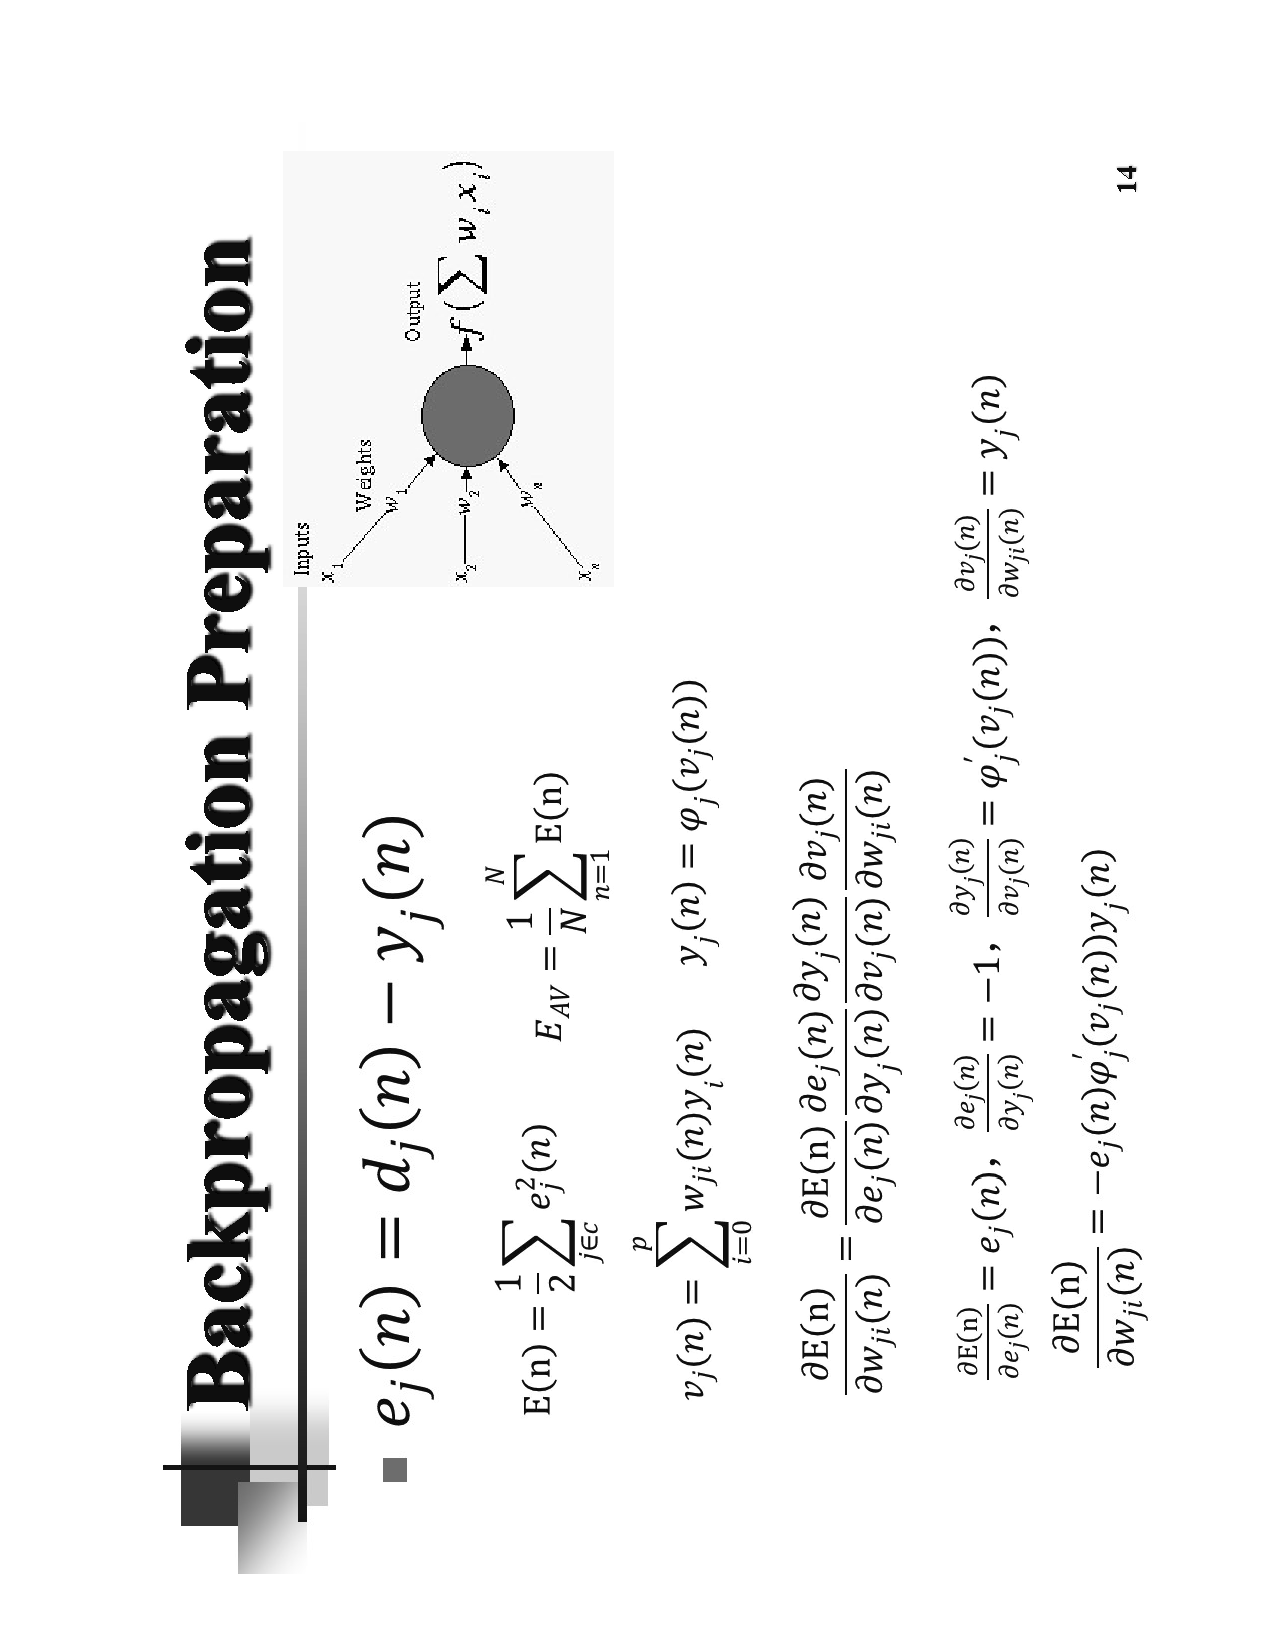
\includegraphics[height=\columnwidth,angle = -90]{NN/5.pdf}
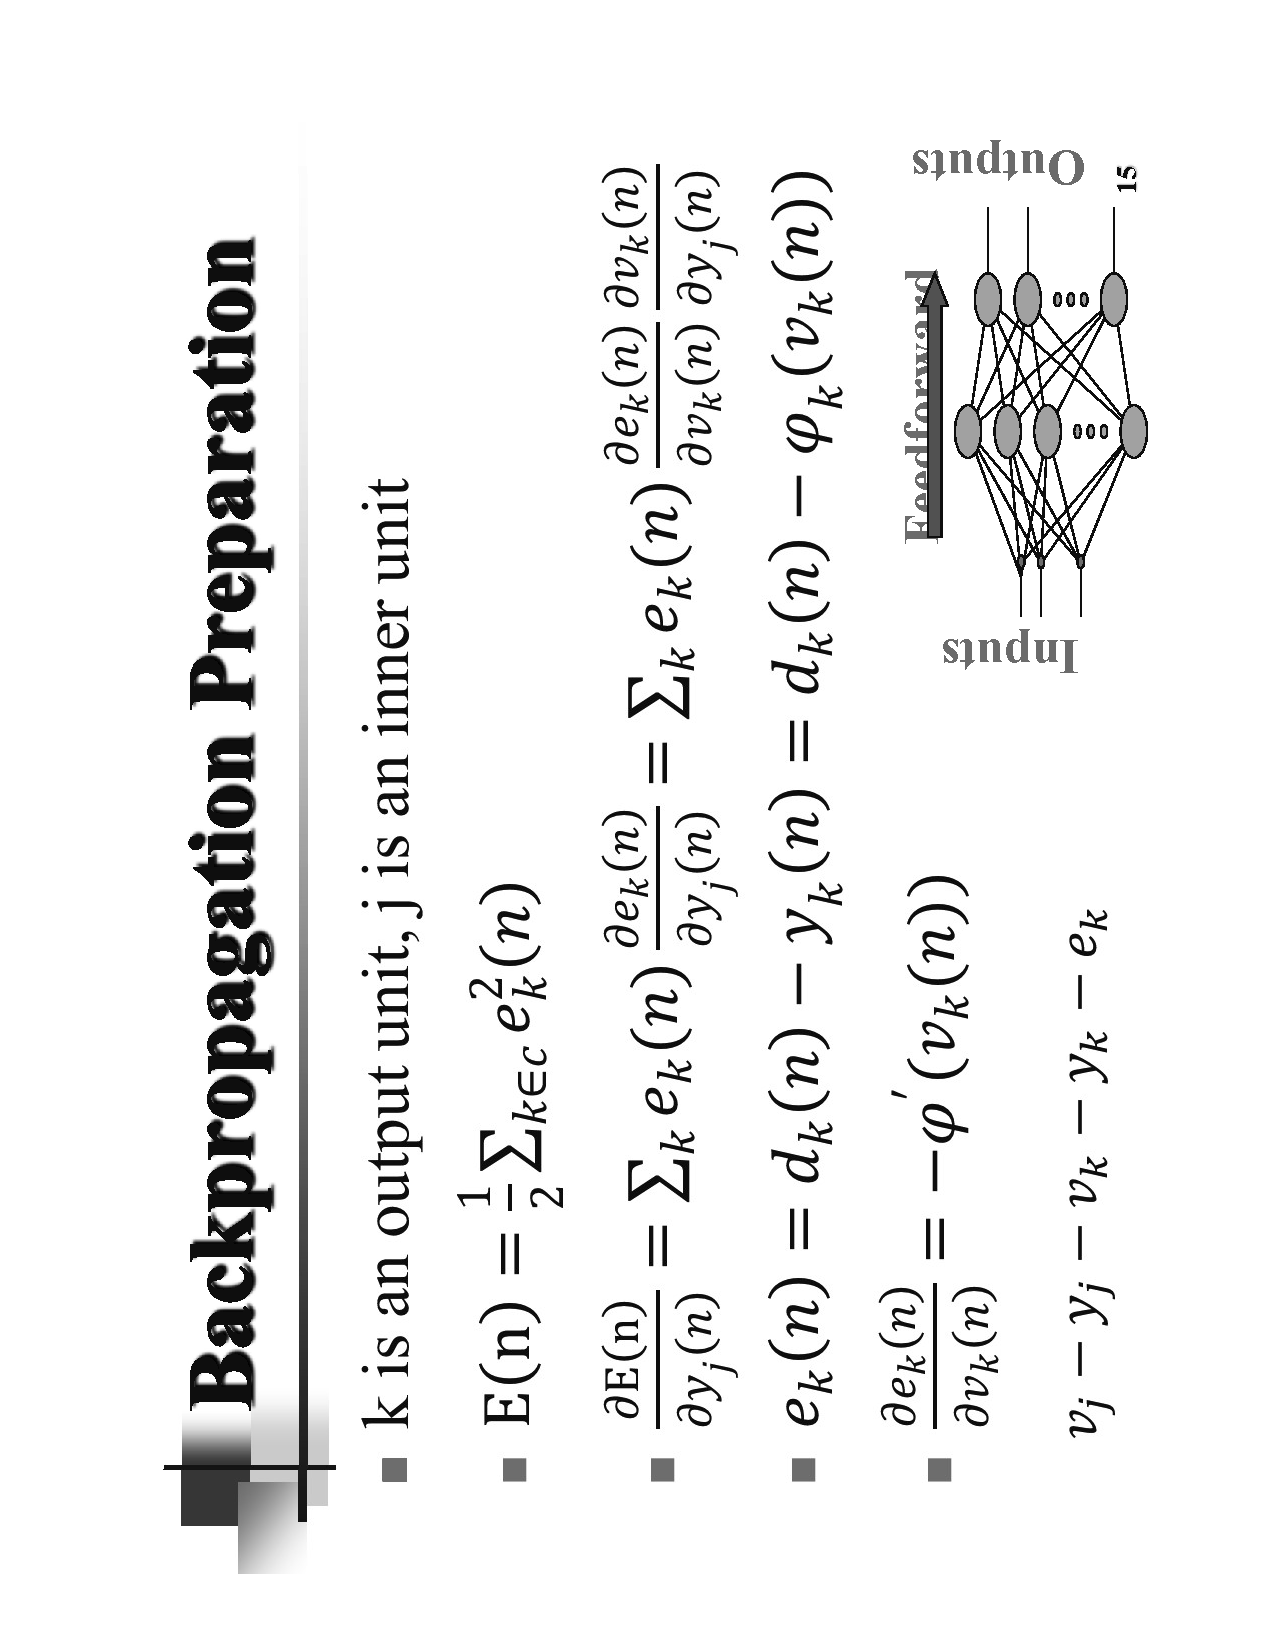
\includegraphics[height=\columnwidth,angle = -90]{NN/6.pdf}
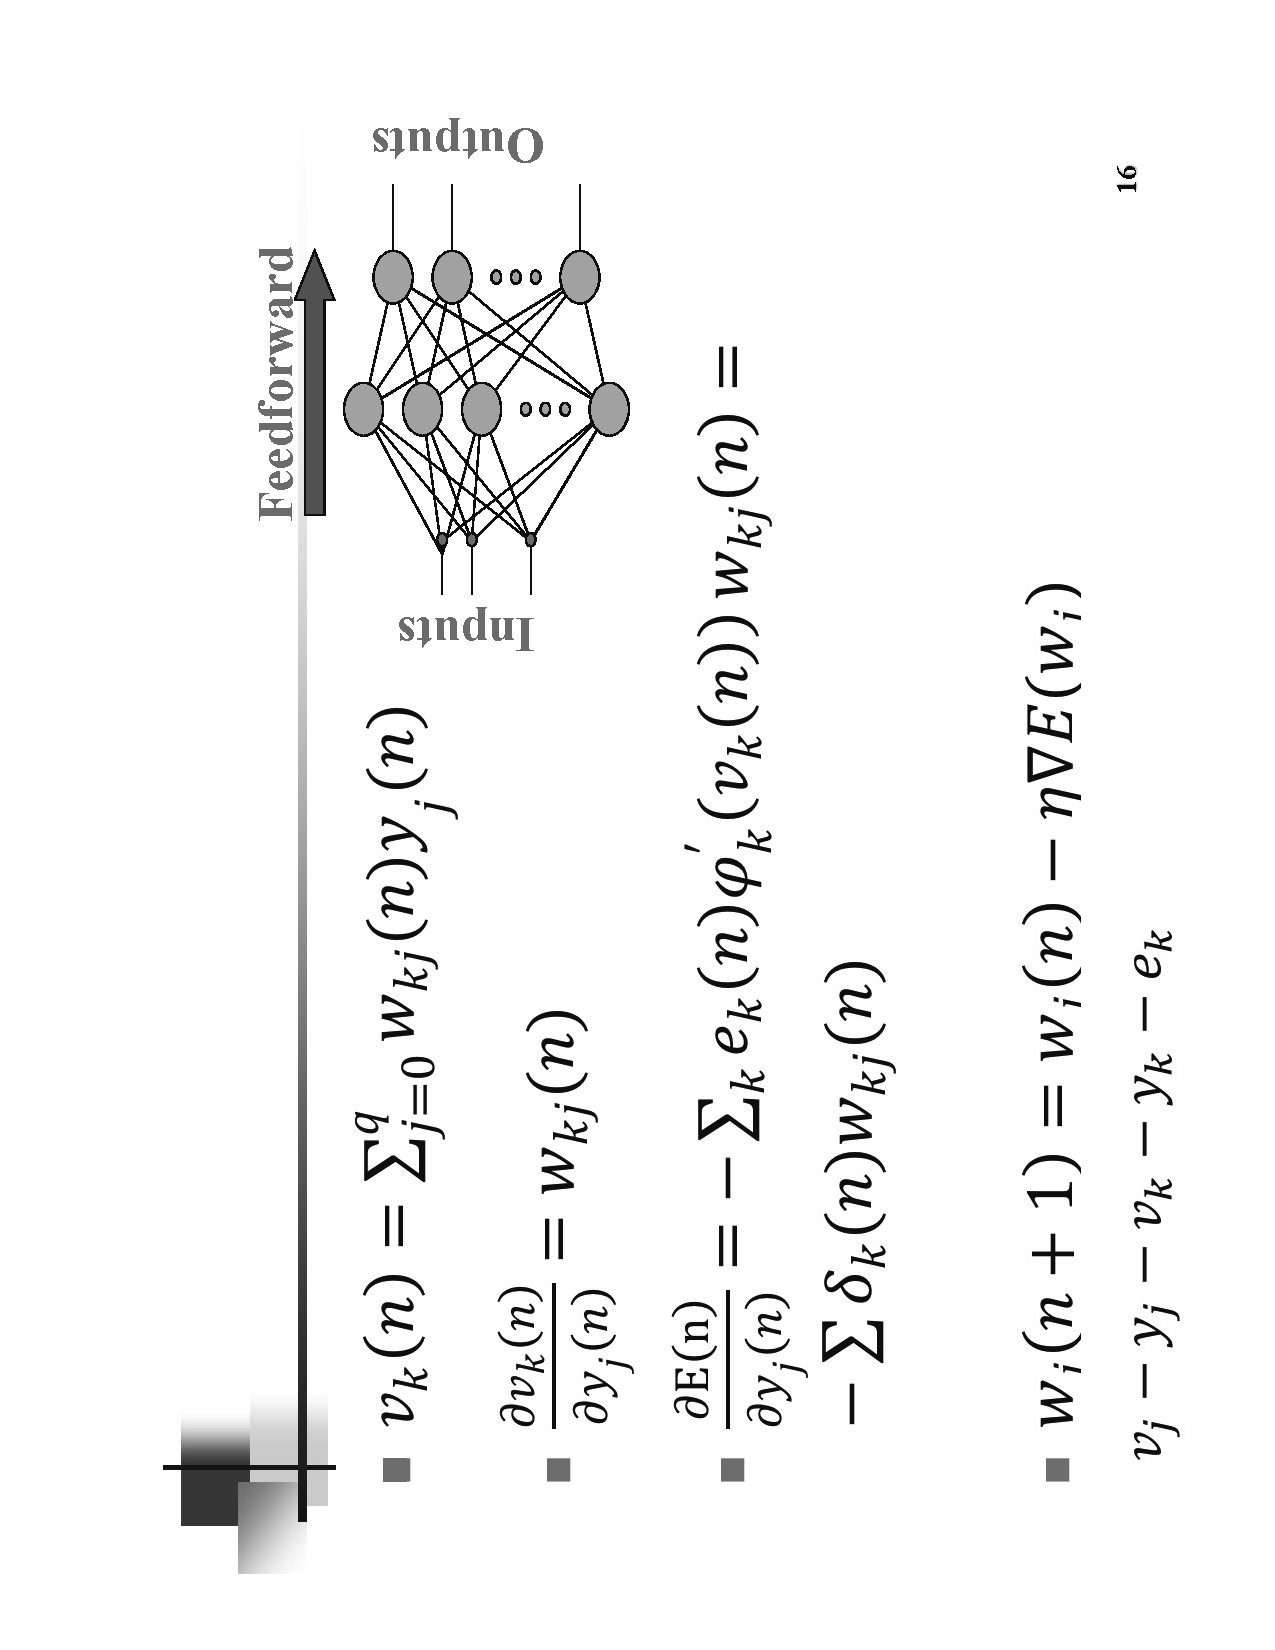
\includegraphics[height=\columnwidth,angle = -90]{NN/7.pdf}
\end{figure}
\noindent BP应用:采用Re\_LU激活函数,交叉熵。统计batch梯度下降,随机抽取训练集(非常重要),输入标准化(零均值1方差),调整学习步长,使用dropout降低过拟合

\noindent 训练过程:随机初始化权重,当训练误差大于目标时:\\
\noindent 训练样本,得到输出和输出误差,反向传播等\\
\noindent 最后测试神经网络性能。

\noindent CNN 结构:卷积,池化,全连接.Le-Net5结构,【输入】1@32*32【卷积】6@28*28【池化】6@14*14【卷积】12@10*10【池化】12@5*5【全连】100@1*1【全连】10【输出】

\noindent CNN适用于:信号以数组方式接受。信号有强的局部关联性,信号特征可能出现在任何位置。

\noindent 1D:时间序列分析,文本。2D:音频,图片。3D:视频
\begin{figure}[H]
\centering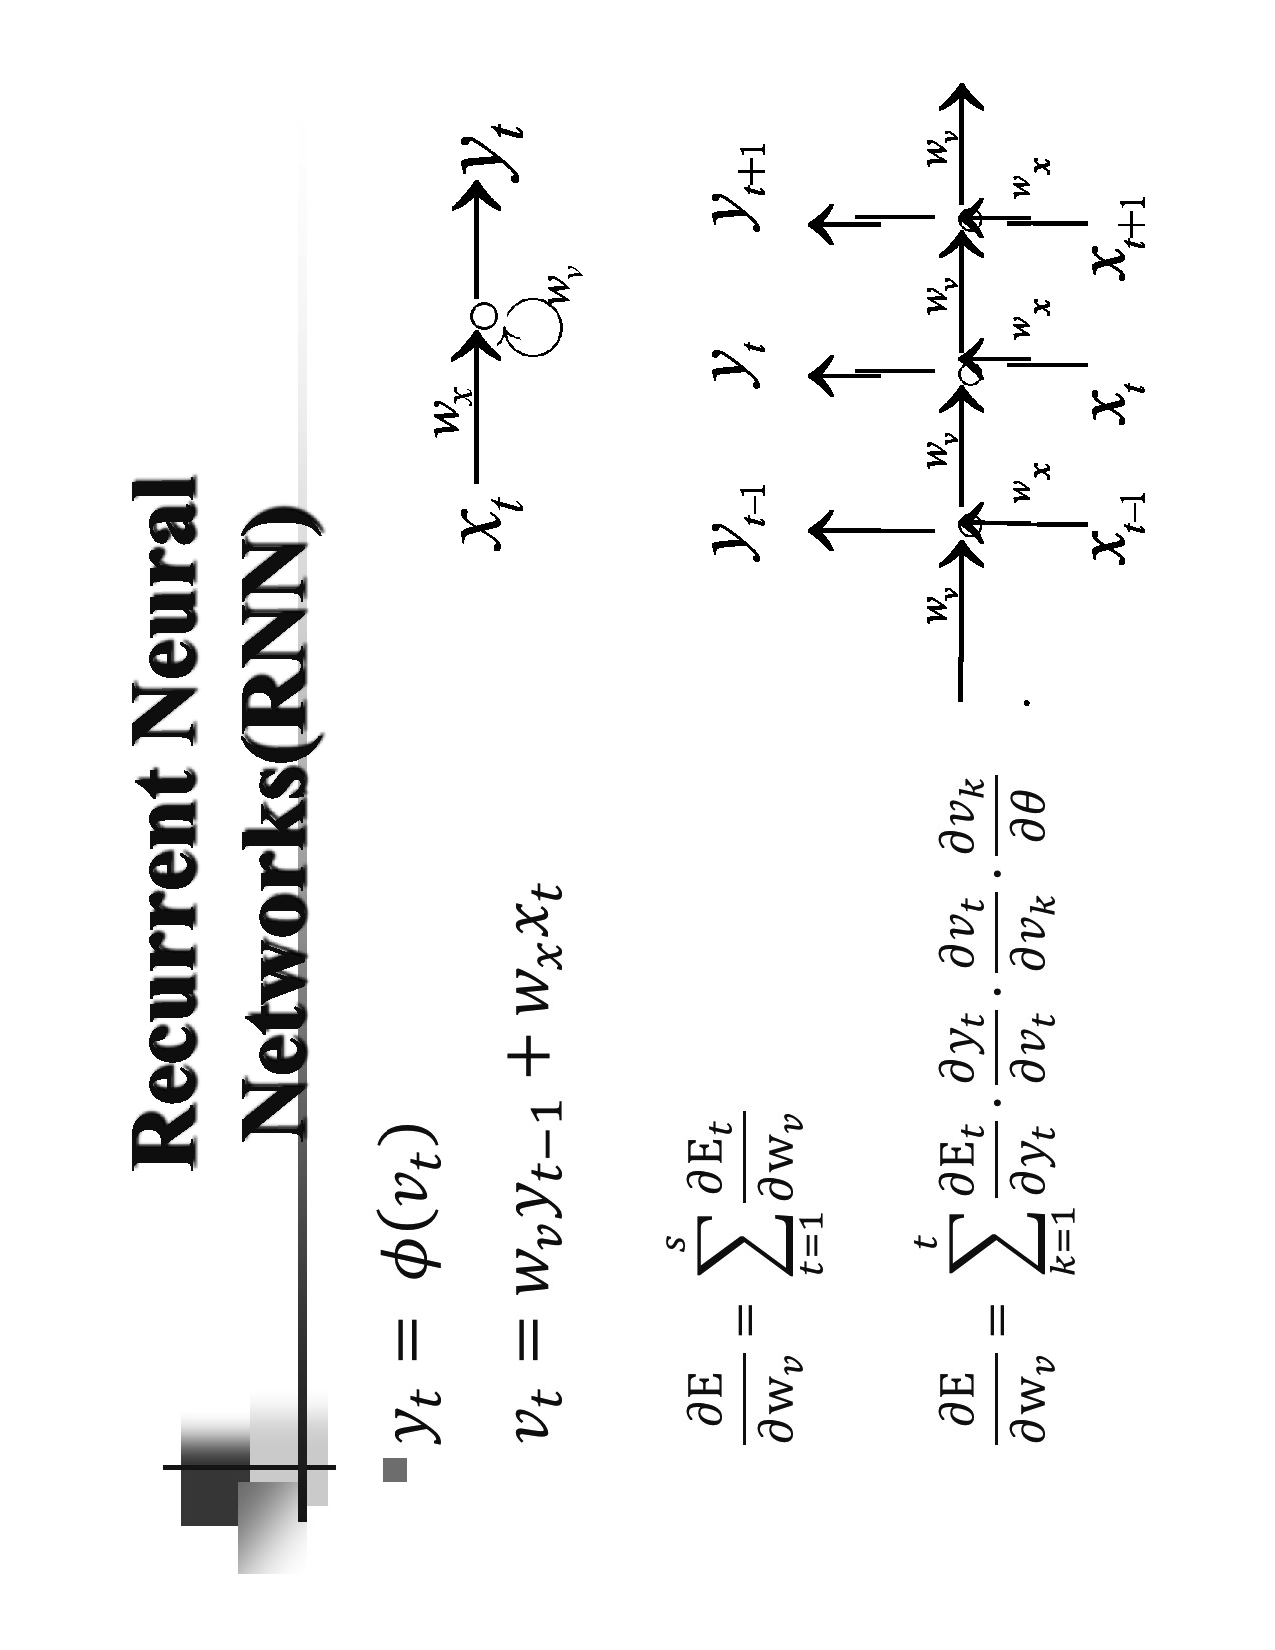
\includegraphics[height=\columnwidth,angle = -90]{NN/12.pdf}
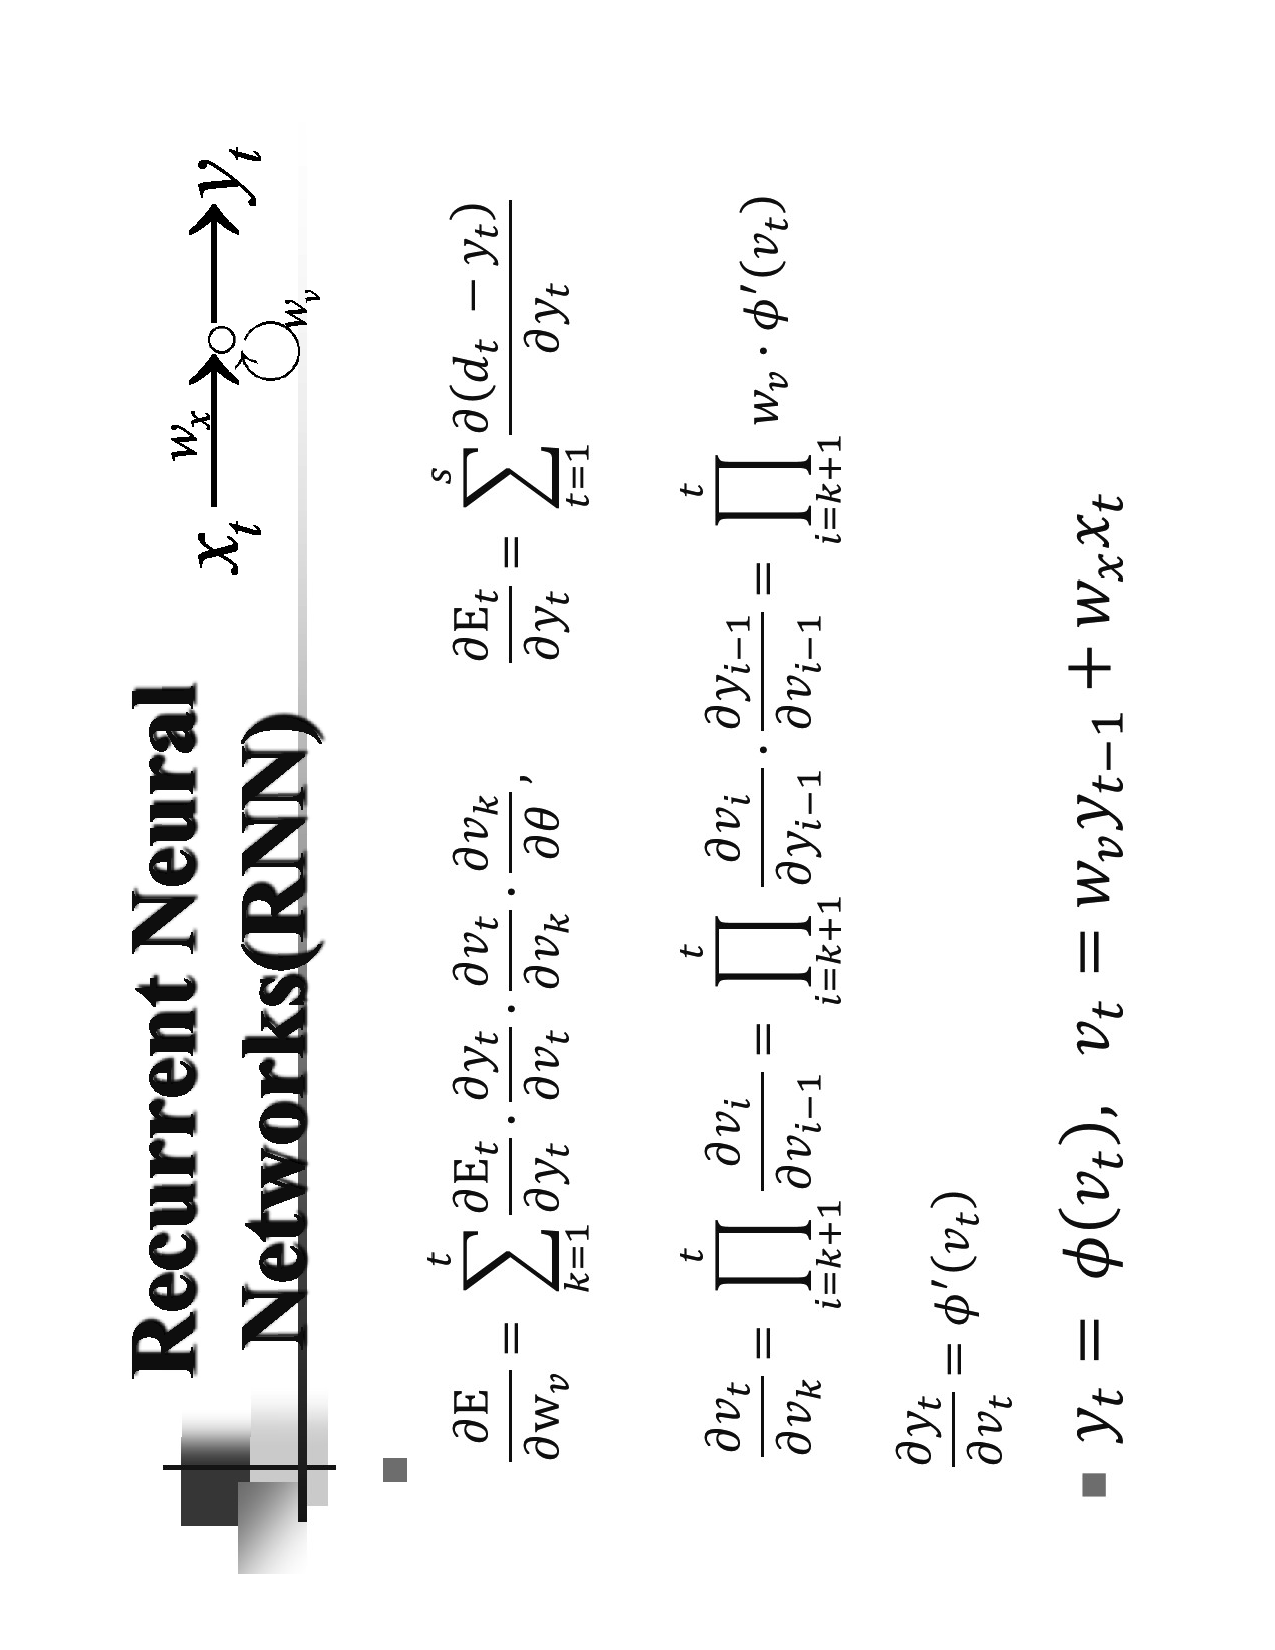
\includegraphics[height=\columnwidth,angle = -90]{NN/13.pdf}
\end{figure}
\begin{figure}[H]
\centering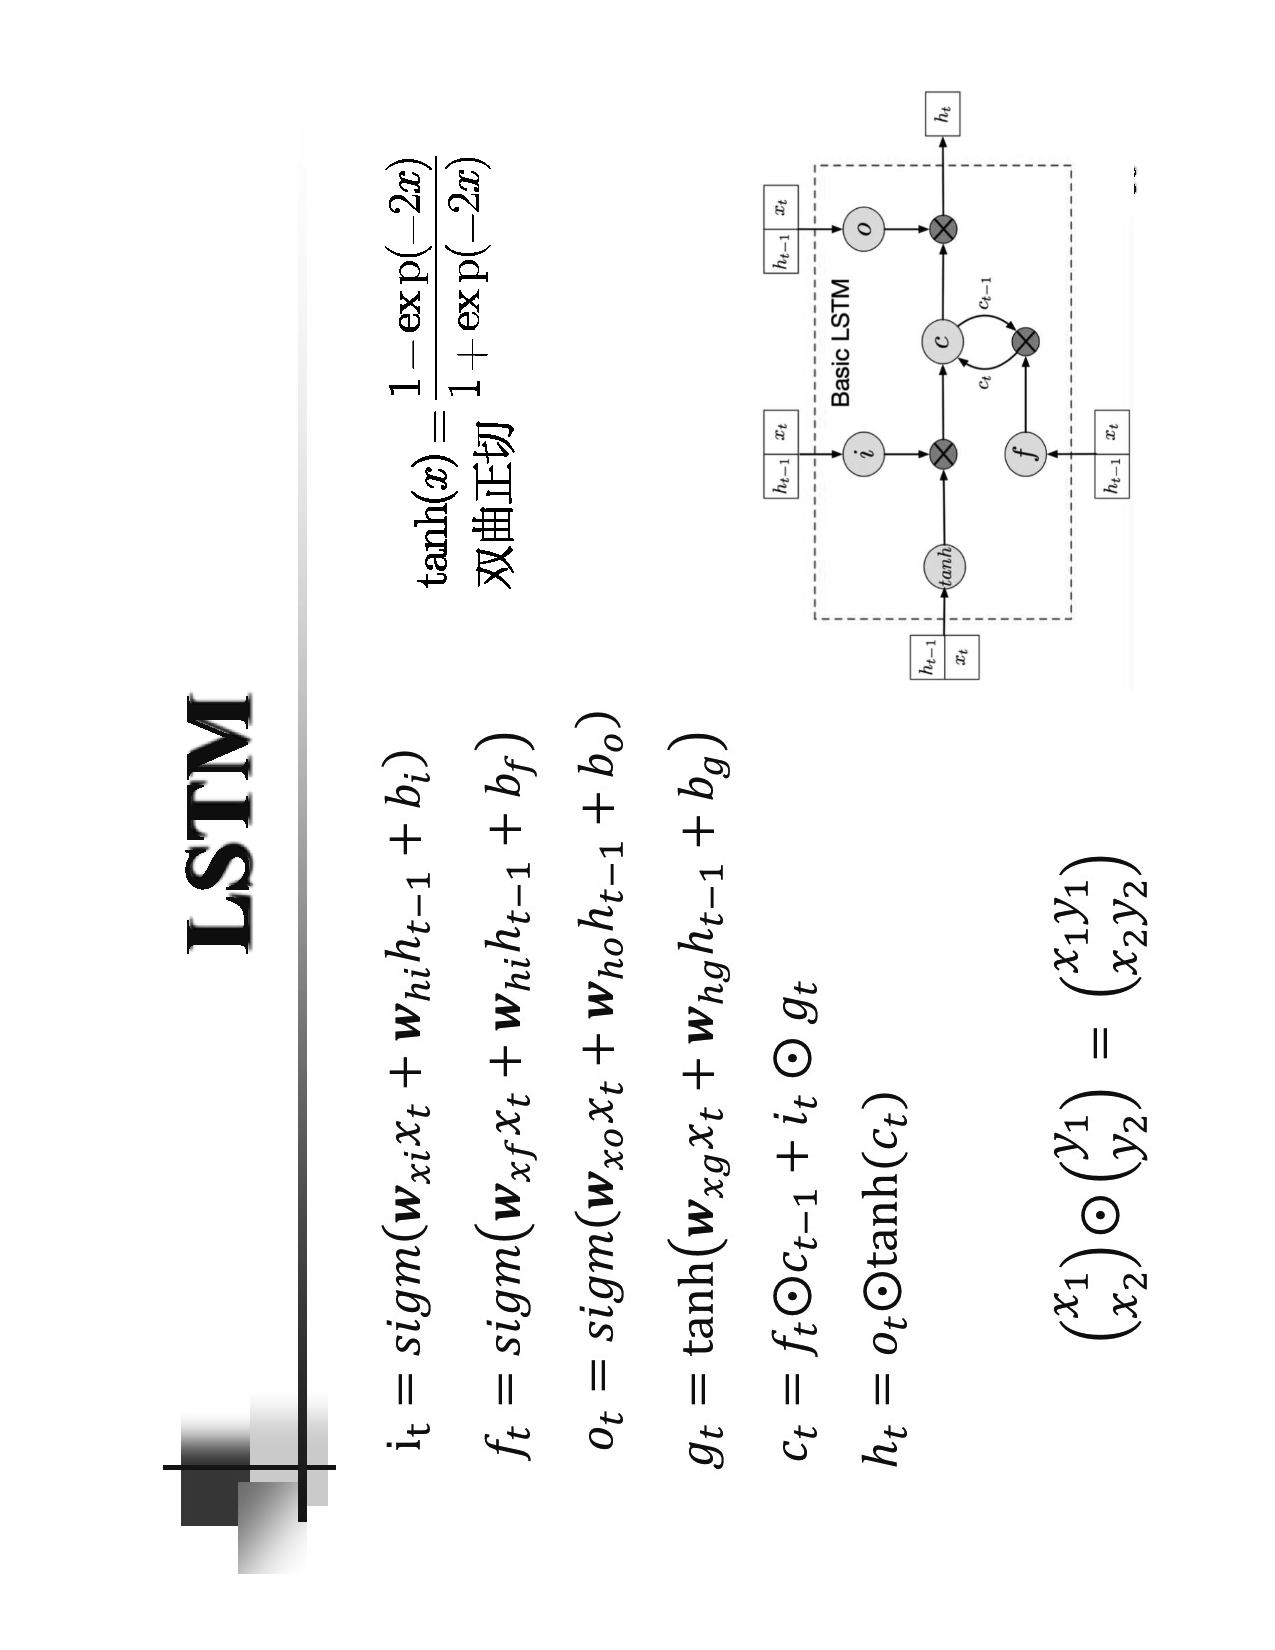
\includegraphics[height=\columnwidth,angle = -90]{NN/14.pdf}
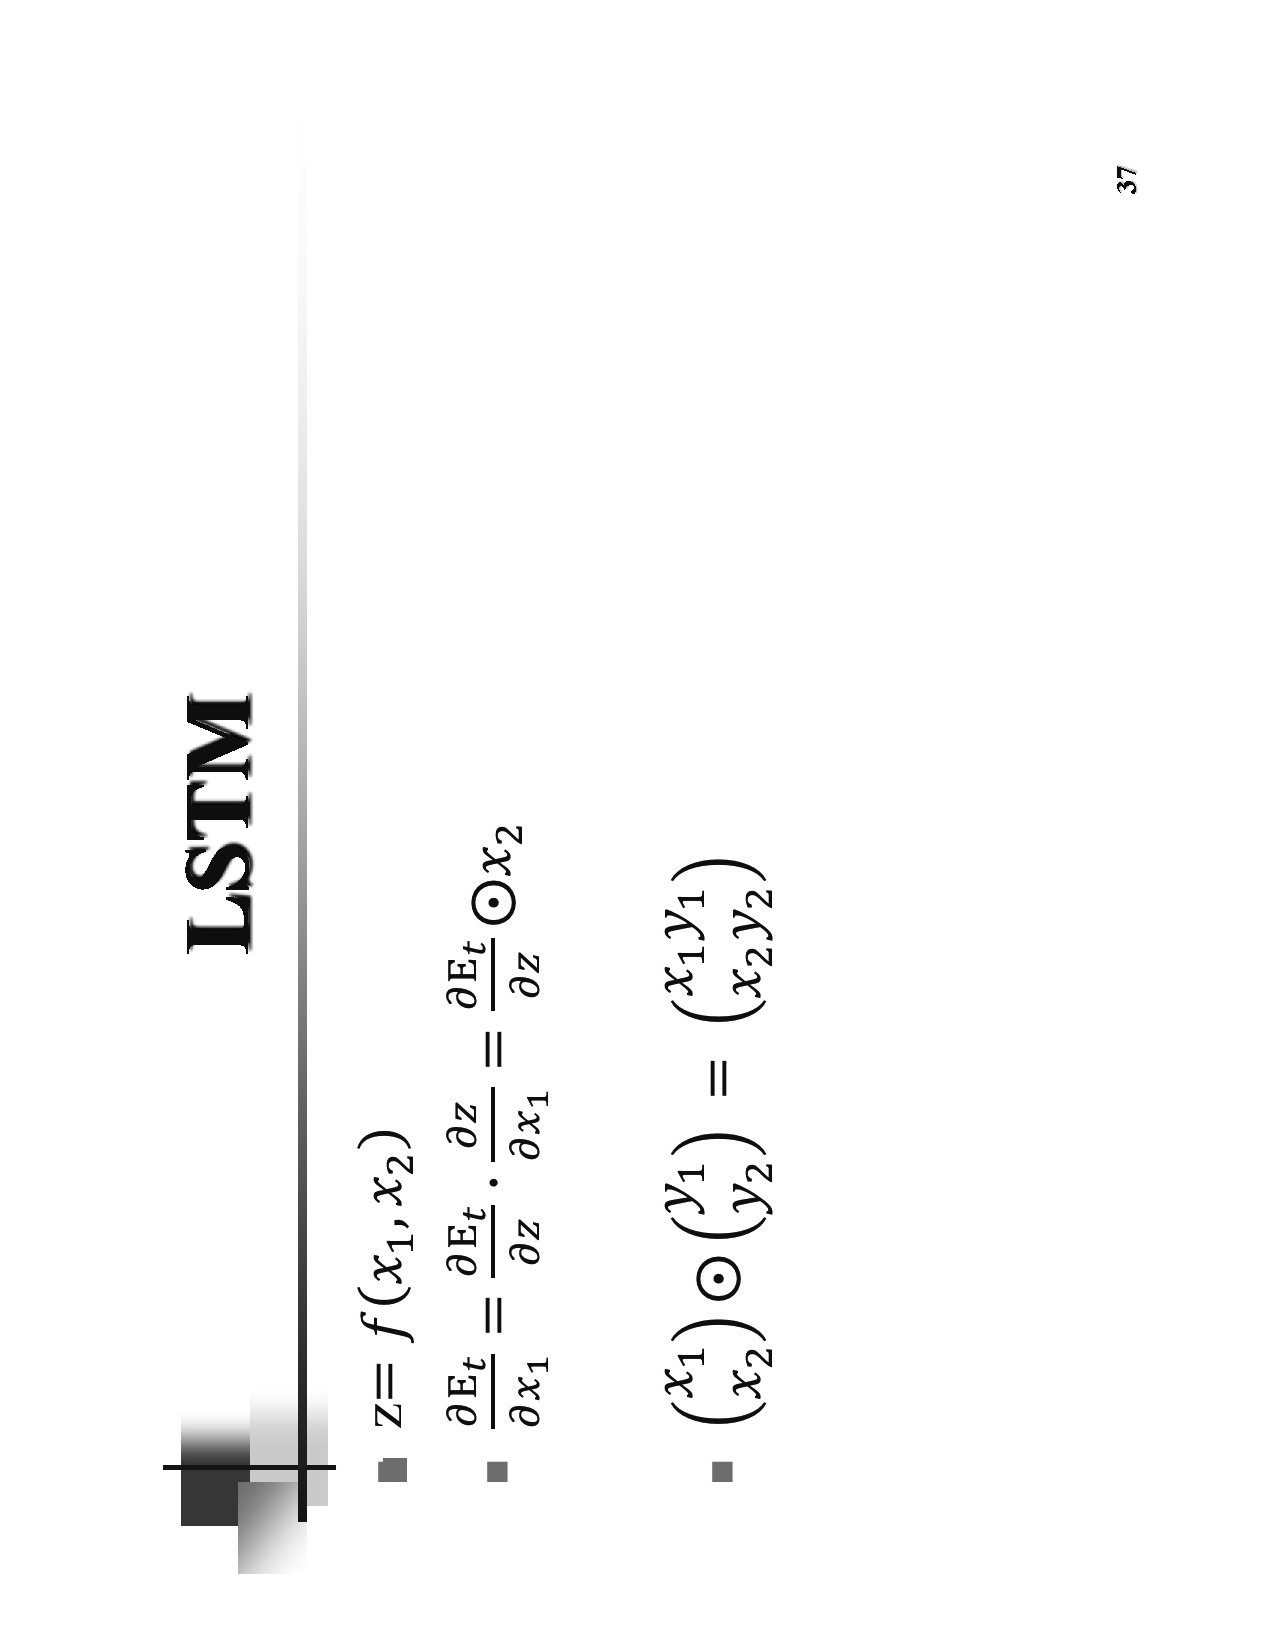
\includegraphics[height=\columnwidth,angle = -90]{NN/15.pdf}
\end{figure}
\noindent 感知机(Perceptron)$$x = [x_{1} x_{2} ...x_{p}]^{T}, x_{j}\in R,w = [w_{1} w_{2} ...w_{p}]^{T}, w_{j}\in R$$$$v  = \sum_{i=i}^p w_{i}x_{i}-\theta=W^{T}X - \theta,y = sgn(v)$$

\noindent 输出:Sigmoid Function $$f(x)=\frac{1}{1+e^{-\lambda x}}$$
Rectification,Piecewise linear, linear function, perceptron, work flow

\noindent 多层神经网络的任意逼近能力

\noindent Classification:Binary classification,  1 output unit: y=0 or 1,  Multi-class classification,  K output units
\end{multicols}
\end{document}